\documentclass{beamer}
\usepackage[utf8]{inputenc}
\usepackage[english]{babel}
\usepackage[T2A]{fontenc}
\usepackage{amsmath}
\usepackage{amsfonts}
\usepackage{amsthm}
\usepackage{bbm}
\usepackage{amssymb}
\usepackage{bm}
\usepackage{graphicx}
\usepackage{epstopdf}
\usepackage[]{algorithm2e}
\usepackage{amsthm}
\usepackage{float}
\usepackage{caption}
%\usetheme{Warsaw}
%\usecolortheme{sidebartab}
\usetheme{Warsaw}
\usecolortheme{seahorse}

%\definecolor{beamer@blendedblue}{RGB}{255,255,0}
%\definecolor{beamer@blendedblue}{HTML}{008A34} %green
%\definecolor{beamer@blendedblue}{HTML}{4A4A4A} %grey
%\definecolor{beamer@blendedblue}{HTML}{0E9059} %biryuz
\definecolor{beamer@blendedblue}{HTML}{027466} %blue


\theoremstyle{definition}
\newtheorem{defin}{Definition}
\newtheorem{assumption}{Assumption}
\theoremstyle{plain}
\newtheorem{thm}{Theorem}
\newtheorem{lem}{Lemma}
\newtheorem{prop}{Proposition}
\theoremstyle{remark}
\newtheorem{remark}{Remark}
\newtheorem{prob}{Problem}
\def\eqdef{\stackrel{def}{=}}

% \DeclareMathOperator*{\argmin}{argmin}
% \DeclareMathOperator*{\Argmin}{Argmin}
% \DeclareMathOperator{\barcnt}{bar}
% \DeclareMathOperator{\supp}{supp}
% \DeclareMathOperator{\est}{\mathbb{E}}
% \DeclareMathOperator{\inter}{int}
% \DeclareMathOperator{\ind}{Ind}

\begin{document}
\setlength{\abovedisplayskip}{5pt}
\setlength{\belowdisplayskip}{5pt}

	\title[\hbox to 60mm{High-dimensional integrals \hfill\insertframenumber\,/\,10}]
			{ Course project \\ <<High-dimensional integrals for option pricing>>}
	\author[A. Podkopaev, N. Puchkin, I. Silin]{\large Alexander Podkopaev, Nikita Puchkin, Igor Silin \\Team <<Spokoynye>>}
	\institute[Affiliation]{
	\textsc{Skolkovo institute of science and technology}
	}

\date{\footnotesize{December 16, 2016}}

	\begin{frame}
		\titlepage
	\end{frame}

	\begin{frame}{Plan}
		  \tableofcontents[
		    sectionstyle=show/show,
		    subsectionstyle=show/show/show
		  ]
	\end{frame}
	
	\section{Introduction to option pricing }
	\begin{frame}{Introduction to option pricing}	 
		\begin{block}{Options}
			\begin{itemize}
				\item Contract which gives the owner of the option the right, but not the obligation, to buy or sell an underlying asset at a specified price on a specified date, depending on the form of the option
				\item Two basic types of options: the call and the put
				\item Call -  gives the holder the right to buy an asset 
				\item Put - gives the holder the right to sell an asset
			\end{itemize}
		\end{block}
		\begin{block}{Notations}
			\begin{itemize}
				\item $s$ - stock price 
				\item $c(s,t)$ - general option value
			\end{itemize}
		\end{block}	 
	\end{frame}

	\section{From Black-Scholes to diffusion }

		\begin{frame}{Black-Scholes equation}
			\vspace{-5pt}
			\begin{block}{Black-Scholes equation}
				\begin{equation}
					\begin{aligned}
						&\frac{\partial c(s,t)}{\partial t} +
						rs \frac{\partial c(s,t)}{\partial s} +
						\frac12 \gamma^2 s^2 \frac{\partial^2 c(s,t)}{\partial s^2} =
						rc(s,t),\\
						&c(s,T^{\prime}) = g(s), \;\;\;\;\; s \in \mathbbm{R}_{+},\\
						&c(0,t) = 0, \;\;\;\;\;\;\;\;\;\;\;\; t \in [0;\;T^{\prime}].
						\nonumber
					\end{aligned}
				\end{equation}
			\end{block}

			\vspace{-5pt}
			\begin{block}{Substitution}
						\begin{itemize}
							\item New variable: $x=\ln s$
							\item New initial condition: $f(x) = e^{\frac{1}{\gamma^2} (r-\frac{\gamma^2}{2})x} g(e^x)$,
							\item New coefficients: $\sigma = \frac12 \gamma^2$,
						 			$V(x,t) = V = r +  \frac{1}{2\gamma^2} \left( r-\frac{\gamma^2}{2}\right)^2$,
						 	%\item New soluton: $c(s,t) = e^{-\frac{1}{\gamma^2} (r-\frac{\gamma^2}{2})\ln s} u(\ln s, T^{\prime} - t)$.
						 	\item New solution: $u(x,t) =  e^{\frac{1}{\gamma^2} (r-\frac{\gamma^2}{2})x} c(e^x, T^{\prime} - t)$
						\end{itemize}
			\end{block}
							
		\end{frame}

		\begin{frame}{Diffusion equation}

			\begin{block}{One-dimensional reaction-diffusion equation}
				\begin{equation}
					\begin{aligned}
						&\frac{\partial u(x,t)}{\partial t} = \sigma \frac{\partial^2 u(x,t)}{\partial x^2} - V(x,t) u(x,t),
						\;\;\; t \in [0;\;T^{\prime}],\\
						&u(x,0) = f(x), \;\;\; x \in \mathbbm{R}.
					\nonumber
					\end{aligned}
				\end{equation}
			\end{block}

			\begin{center}
				Fast method for solving this equation was proposed in the paper:\\
				''A low-rank approach to the computation of path integrals'',\\ M. Litsarev, I. Oseledets, 2015.
			\end{center}
		\end{frame}

	\section{Idea of the method}
		\begin{frame}{Idea of the method}
            \begin{itemize}
                \item The analytical solution is given by the Feynman-Kac formula
                \begin{equation}
                    \begin{aligned}
                    \nonumber
                    u(x, T) = \int\limits_{C\{x,0; T\}} f(\xi(T)) e^{-\int\limits_0^T V(\xi(\tau), T - \tau) d\tau} \mathcal D_\xi
                    \end{aligned}
                \end{equation} 
                \item Time discretization reduces this formula to n-dimensional integral ($n \gg 1$)
                \item But it can be computed as $n$ one-dimensional convolutions efficiently  
                \item Сonvolutions can be computed efficiently via FFT or/and low-rank approximations
            \end{itemize}		
		\end{frame}
		

	\section{Experiments}
						
		\begin{frame}{Experiments: european put option}
		
				 	Terminal conditions:
		 \[
			g(s)=\max\{ E-s,0 \}	 
		 \]	
			\begin{minipage}{\linewidth}
      \centering
      \begin{minipage}{0.45\linewidth}
          \begin{figure}[H]
              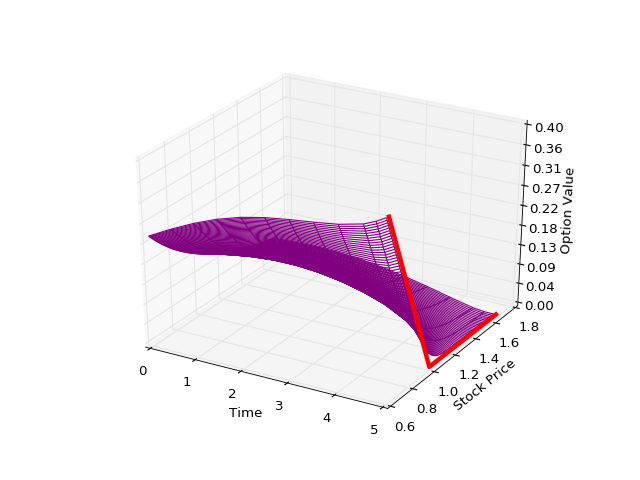
\includegraphics[width=\linewidth]{Figures/eu-put}
              \caption{Numerical solution}
          \end{figure}
      \end{minipage}
      \hspace{0.05\linewidth}
      \begin{minipage}{0.45\linewidth}
          \begin{figure}[H]
              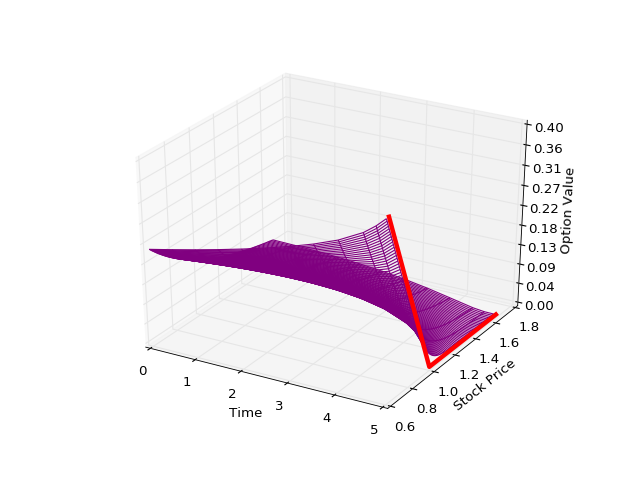
\includegraphics[width=\linewidth]{Figures/eu-put-analyt}
              \caption{Analytical solution}
          \end{figure}
      \end{minipage}
  \end{minipage}
 	\end{frame}

		\begin{frame}{Experiments: Cash-or-nothing call option}
		
				 Terminal conditions:	 
		 \[
			g(s)=\begin{cases} B, & s\geq E \\
			0, & s< E \end{cases}
		 \]	
\begin{minipage}{\linewidth}
      \centering
      \begin{minipage}{0.45\linewidth}
          \begin{figure}[H]
              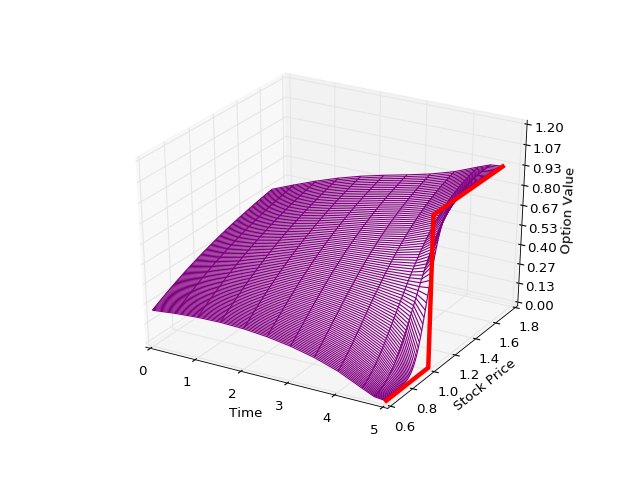
\includegraphics[width=\linewidth]{Figures/c-o-n-call}
              \caption{Numerical solution}
          \end{figure}
      \end{minipage}
      \hspace{0.05\linewidth}
      \begin{minipage}{0.45\linewidth}
          \begin{figure}[H]
              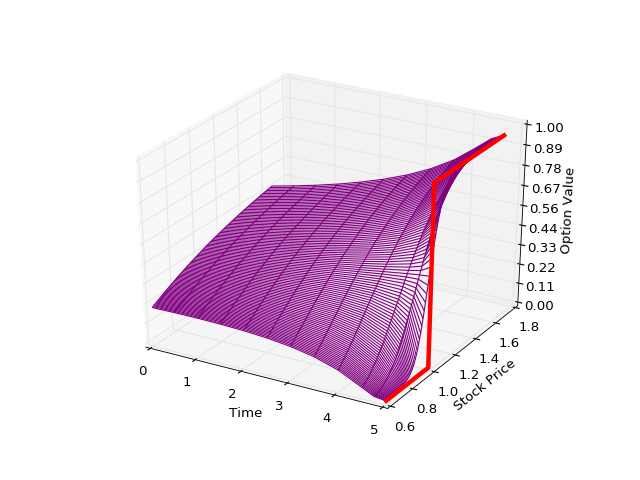
\includegraphics[width=\linewidth]{Figures/c-o-n-call-analyt}
              \caption{Analytical solution}
          \end{figure}
      \end{minipage}
  \end{minipage}	 	 
		\end{frame}
		
	\section{Discussion}

		\begin{frame}{Discussion}
			\vspace{-7pt}
			\begin{block}{Unbounded terminal condition}
				\begin{itemize}
					\item If $n$ is big, numerical solution $\rightarrow +\infty$.\\
					Explanation: \\substitution $x = \ln s$ and one speciality of the algorithm.
					\item If $n$ is small, numerical solution is not accurate and cross approximation is not useful.
				\end{itemize}
			\end{block}
			\vspace{-3pt}
			\begin{block}{Bounded terminal condition}
				\begin{itemize}
					\item No such failure with big $n$ as in the previous case.
					\item The bigger $n$, the more accurate solution.
					\item Cross approximation is useful: allows to reduce complexity.
				\end{itemize}
			\end{block}
			\centering{More detailed analysis on that in our report.}
		\end{frame}
	
	\section*{}

		\begin{frame}{}
			\centering{ \LARGE Thanks for your attention!}
		\end{frame}

\end{document} 